%
% fundamentallemma.tex -- Beweis des Fundamentallemmas
%
% (c) 2024 Prof Dr Andreas Müller
%
\begin{figure}
\centering
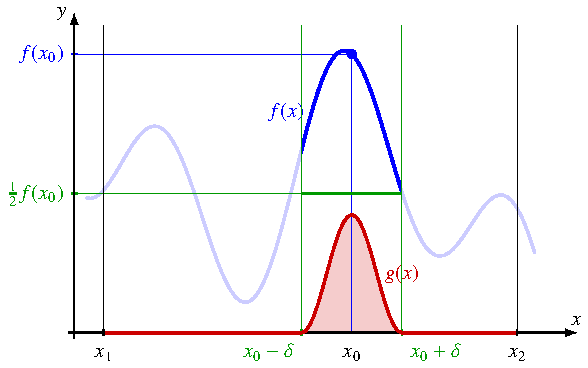
\includegraphics{chapters/020-variation/images/fundamentallemma.pdf}
\caption{Beweis des Fundamentallemmas: Falls $f(x_0)>0$ ist, gibt es
eine Umgebung $[x_0-\delta,x_0+\delta]$, in der immer noch
$f(x)>\frac12f(x_0)$ gilt und eine Funktion $g(x)$ die genau in diesem
Intervall $\ge 0$ ist und ausserhalb verschwindet.
Es folgt, dass das Ingegral $\int_{x_1}^{x_2} f(x)g(x)\,dx>0$ ist
im Widerspruch zur Annahme des Fundamentallemmas.
\label{buch:variation:fundamentallemma:fig:beweis}}
\end{figure}
